
\section{Hardware Components}
\subsection{Robot Platform}
\hspace{2cm}The platform we use in our project is 6-wheel-drive chassis from Dagu Electronics has independent suspension for each of its spiked 120mm-diameter wheels, allowing exceptional traction over uneven terrain, and its body is made from 2mm-thick anodized aluminum with a 10mm-pitch grid of 4mm holes, making it easy to mount electronics and accessories to the chassis. Assembly of the chassis is a simple three-step process that takes just minutes. This model has 75:1 steel gearboxes on the motors, see figure \ref{fig:wild thumper}. The robot the following architecture: \cite{web012}
 \begin{itemize}
        \item Size: 420 x 300 x 130 mm
        \item Weight: 2.7 kg
        \item Recommended motor voltage: 2 - 7.5 V
        \item Metal gearmotor: 25D mm
        \item Dagu wheel (chrome) with Pololu: 120 x 60 mm
    \end{itemize}{}

 \begin{figure}[H]%
    \center%
    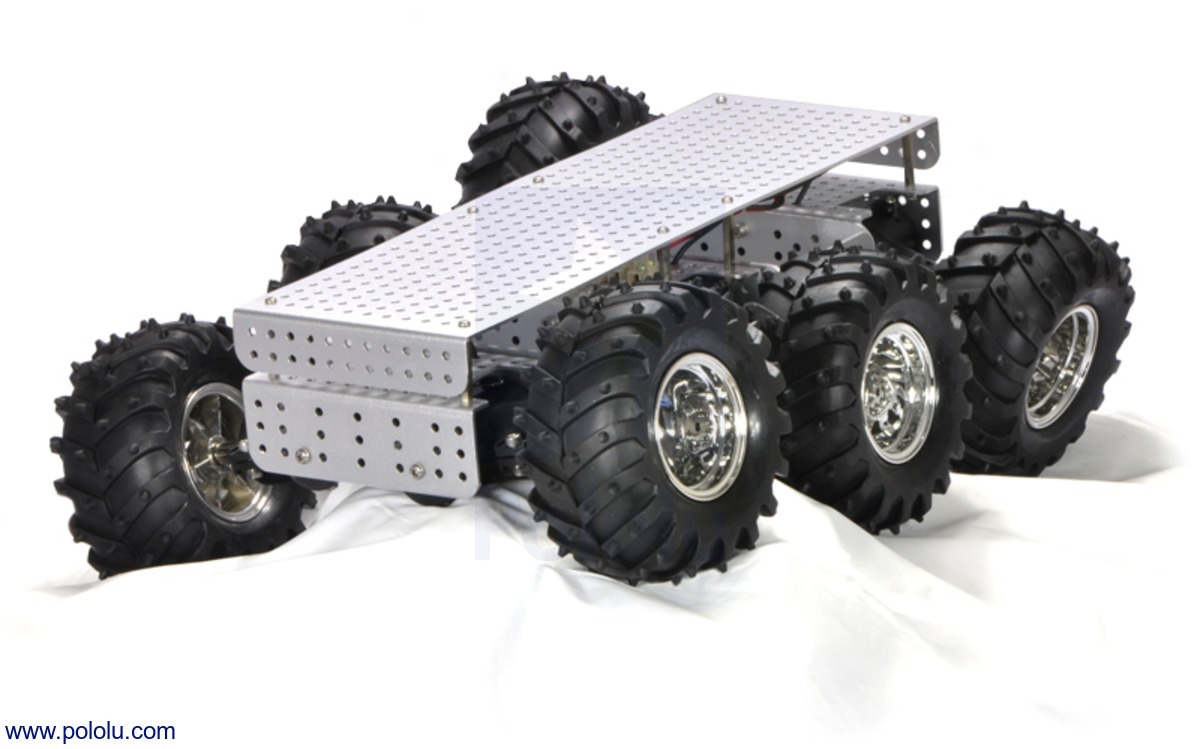
\includegraphics[width=.8\textwidth]
    {images/Alzahraa/wild_thumper.jpg}%
    \caption[Wild Thumper]{Wild Thumper 6 WD}\label{fig:wild thumper}%
  \end{figure} 

\subsection{Motor Drivers}
\hspace{2cm}Motor drives are circuits used to run a motor. In other words, they are commonly used for motor interfacing. These drive circuits can be easily interfaced with the motor and their selection depends upon the type of motor being used and their ratings (current, voltage).\cite{web013}\\
In our project we use two BTS7960 KIT (see figure \ref{fig:motor drivers}) having the following architecture:
\begin{itemize}
    \item High-power drive full H-bridge driver module with thermal over-current protection.  High-current 43A.
    \item Double BTS7960 large current (43 A) H bridge driver.
    \item 5V isolate with MCU, and effectively protect MCU.
    \item 5V power indicator on board.
    \item Voltage indication of motor driver output end.
    \item Heat sink can be added. 
    \item Isolation chip 5 V power supply (can share with MCU 5 V).
    \item Size: 4 * 5 * 1.2 cm.
    \item Ability to reverse the motor forward, two PWM input frequency up to 25kHZ.
    \item Two heat flow passing through an error signal output.
    \item Isolated chip 5V power supply (can be shared with the MCU 5V), can also use the on-board 5V supply.
    \item The supply voltage 5.5V to 27V. 
\end{itemize}
Both drivers are powered by LIPO 7.4V -4200mAh battery.

\begin{figure}[H]%
    \center%
    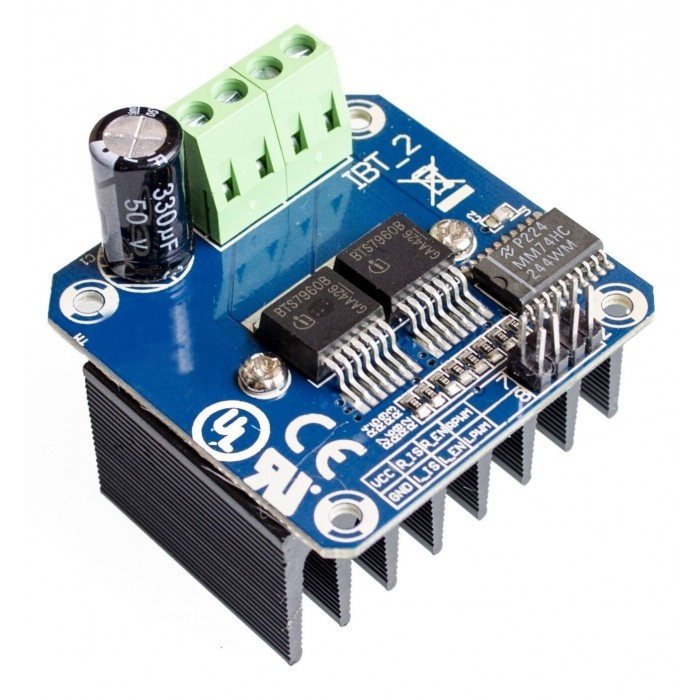
\includegraphics[width=.5\textwidth]
    {images/Alzahraa/motor_drivers.jpg}%
    \caption[Motor Driver]{Motor driver BTS7960}\label{fig:motor drivers}%
  \end{figure} 

\subsection{Arduino}
\hspace{2cm}Arduino is an open-source hardware and software company, project and user community that designs and manufactures single-board microcontrollers and microcontroller kits for building digital devices and interactive objects that can sense and control both physically and digitally.
Arduino board designs use a variety of microprocessors and controllers. The boards are equipped with sets of digital and analog input/output (I/O) pins that may be interfaced to various expansion boards or breadboards (shields) and other circuits. The boards feature serial communications interfaces, including Universal Serial Bus (USB) on some models, which are also used for loading programs from personal computers. The microcontrollers are typically programmed using a dialect of features from the programming languages C and C++. In addition to using traditional compiler toolchains, the Arduino project provides an integrated development environment (IDE) based on the Processing language project.\cite{web017} 
In our project we use Arduino UNO (see figure \ref{fig:arduino uno}) having the following architecture: \\
\begin{itemize}
    \item Microcontroller board based on the ATmega328P.
    \item 14 digital input/output pins (of which 6 can be used as PWM outputs), 6 analog inputs, a 16 MHz quartz crystal, a USB connection, a power jack, an ICSP header and a reset button.\cite{web014}\\
\end{itemize}
\begin{figure}[H]%
    \center%
    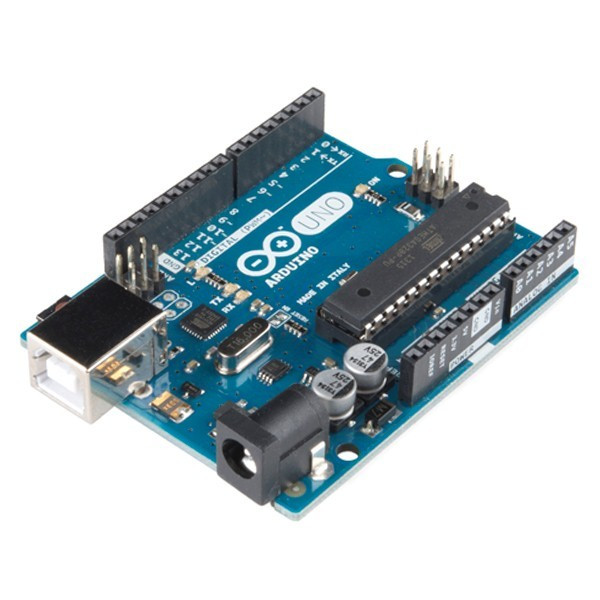
\includegraphics[width=.5\textwidth]
    {images/Alzahraa/arduino_uno.jpg}%
    \caption[Arduino Uno]{Arduino UNO}\label{fig:arduino uno}%
  \end{figure} 

\subsection{Raspberry Pi}
\hspace{2cm}A Raspberry Pi is a credit card-sized computer originally designed for education, inspired by the 1981 BBC Micro. Creator Eben Upton’s goal was to create a low-cost device that would improve programming skills and hardware understanding at the pre-university level. But thanks to its small size and accessible price, it was quickly adopted by tinkerers, makers, and electronics enthusiasts for projects that require more than a basic microcontroller.
The Raspberry Pi is slower than a modern laptop or desktop but is still a complete Linux computer and can provide all the expected abilities that implies, at a low-power consumption level. \cite{web006} \\
In our project we use Raspberyy Pi 3 model B (see figure \ref{fig:raspberryPi}) having the following architecture:
\begin{itemize}
    \item Quad Core 1.2GHz Broadcom BCM2837 64bit CPU.
    \item 1GB RAM.
    \item BCM43438 wireless LAN and Bluetooth Low Energy (BLE) on board.
    \item 100 Base Ethernet.
    \item 40-pin extended GPIO.
    \item 4 USB 2 ports.
    \item 4 Pole stereo output and composite video port.
    \item Full size HDMI.
    \item CSI camera port for connecting a Raspberry Pi camera.
    \item DSI display port for connecting a Raspberry Pi touchscreen display.
    \item Micro SD port for loading your operating system and storing data.
    \item Upgraded switched Micro USB power source up to 2.5A.\cite{web018}
\end{itemize}

\begin{figure}[H]%
    \center%
    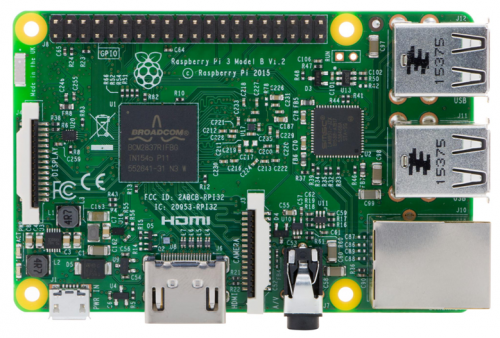
\includegraphics[width=.5\textwidth]
    {images/Alzahraa/raspberryPi.png}%
    \caption[Raspberry Pi]{Raspberry Pi 3 model B}\label{fig:raspberryPi}%
  \end{figure} 


\subsection{Sensors}
\hspace{2cm}A sensor is a device, module, or subsystem whose purpose is to detect events or changes in its environment and send the information to other electronics, frequently a computer processor. \cite{web007} \\
Sensors used in our project are:
\begin{enumerate}
   \item IMU: \\
   An inertial measurement unit (IMU) is an electronic device that measures and reports a body's specific force, angular rate, and sometimes the orientation of the body, using a combination of accelerometers, gyroscopes, and sometimes magnetometers. \cite{web008}\\
   In Our project we use Adafruit 9-DOF IMU module (see figure \ref{fig:fig:adafruit}) having the following architecture:

    \begin{itemize}
        \item Dimensions: 20mm x 27mm x 4mm / 0.8" x 1.1" x 0.2"
        \item Header holes begin 4mm from the mounting holes
        \item Mounting Hole dimensions: 20mm x 12mm apart
        \item Uses I2C address 0x28 (default) or 0x29
        \item Weight: 3g 
    \end{itemize}{}

   \begin{figure}[H]%
    \center%
    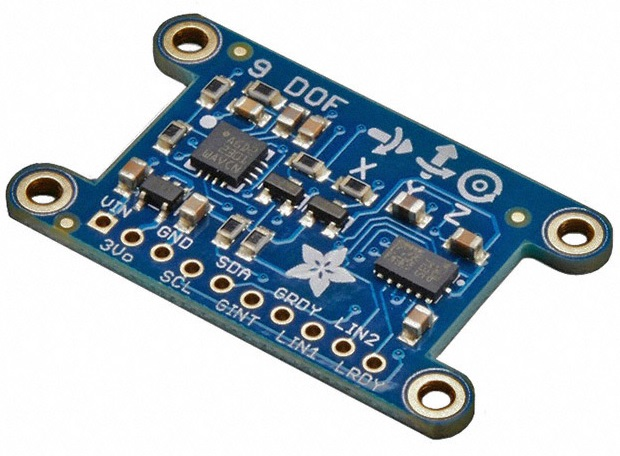
\includegraphics[width=.5\textwidth]
    {images/Alzahraa/imu_Adafruit.jpg}%
    \caption[IMU Adafruit]{Adafruit 9-DOF IMU}\label{fig:adafruit}%
  \end{figure}
   
   \item GPS: \\
   The Global Positioning System (GPS), is a satellite-based radionavigation system owned by the United States government and operated by the United States Air Force. It is a global navigation satellite system that provides geolocation and time information to a GPS receiver anywhere on or near the Earth where there is an unobstructed line of sight to four or more GPS satellites. Obstacles such as mountains and buildings block the relatively weak GPS signals. \cite{web009}\\
   In Our project we use DIYmall NEO-6M GPS module (see figure \ref{fig:neo_6m}) having the following architecture:
    \begin{itemize}
        \item Standalone GPS receiver
        \item U-blox NEO-6M GPS module 
        \item Under 1 second time-to-first-fix for hot and aided starts
        \item SuperSense ® Indoor GPS: -162 dBm tracking sensitivity
        \item Anti-jamming technology
        \item Support SBAS (WAAS, EGNOS, MSAS, GAGAN)
        \item u-blox 6 50 channel positioning engine with over 2 million effective correlators
        \item Timepulse
        \item 5Hz position update rate
        \item Operating temperature range: -40 TO 85°C
        \item UART TTL socket 
        \item EEprom to store settings
        \item Rechargeable battery for Backup 
        \item Build in 18X18mm GPS antenna 
        \item RoHS compliant 
    \end{itemize}{}
     \begin{figure}[H]%
    \center%
    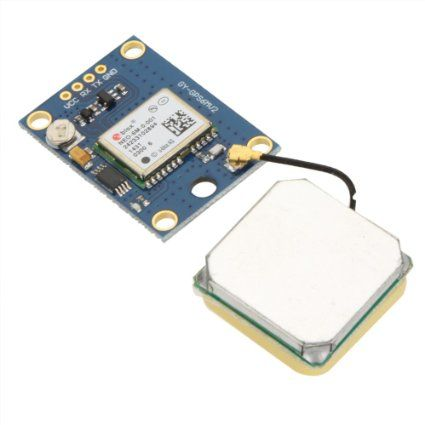
\includegraphics[width=.5\textwidth]
    {images/Alzahraa/gps_NEO_6M.jpg}%
    \caption[GPS NEO]{DIYmall NEO-6M GPS}\label{fig:neo_6m}%
  \end{figure}
   
   \item LIDAR: \\
   Lidar is a surveying method that measures distance to a target by illuminating the target with pulsed laser light and measuring the reflected pulses with a sensor. Differences in laser return times and wavelengths can then be used to make digital 3-D representations of the target. The name lidar, now used as an acronym of light detection and ranging (sometimes light imaging, detection, and ranging), was originally a portmanteau of light and radar. Lidar sometimes is called 3D laser scanning, a special combination of a 3D scanning and laser scanning. It has terrestrial, airborne, and mobile applications. \cite{web010}\\
   In Our project we use YDLIDAR Lidar F4  2D Lidar scanner (see figure \ref{fig:ydlidar}) having the following architecture:
    
    \begin{itemize}
        \item Application field:Environment Scanning, SLAM Application and Robot Navigation
        \item 360-degree laser rangefinder, Scanner range 12 Meter,MAX. 6000Hz Ranging Sample rate
        \item OS: Windows, Android, ROS and Linux,Ultra long working life,Weight: 189g
        \item F4 uses Industrial Brushless Moto,Scanning Rate: 6000tims/s,Laser grade: Class 1,Configurable Scanning Frequency: 5-12Hz
        \item Quick Start-F4 has complete drivers as well as complete SDK ,API and documentation. It's easy for users to get started quickly.
    \end{itemize}{}
    
     \begin{figure}[H]%
    \center%
    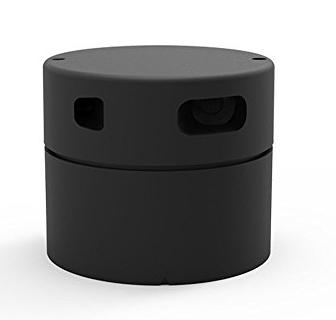
\includegraphics[width=.5\textwidth]
    {images/Alzahraa/lidar_ydlidar.jpg}%
    \caption[YDLIDAR LIDAR]{YDLIDAR Lidar F4  2D Lidar scanner}\label{fig:ydlidar}%
  \end{figure}
   
    \item Webcam: \\
  A webcam is a small digital video camera directly or indirectly connected to a computer or a computer network. \cite{web011}\\
   In Our project we use 1080P Nano Shield N920 Webcamera (see figure \ref{fig:nano_webcam}) having the following architecture:
   
   \begin{itemize}
        \item Premium auto focus and light correction.
        \item Full HD 1080P at 30 fps recording.
        \item Noise cancelling microphone.
        \item Tripod ready mount.
        \item IM compatibility. 
   \end{itemize}{}
   
   \begin{figure}[H]%
    \center%
    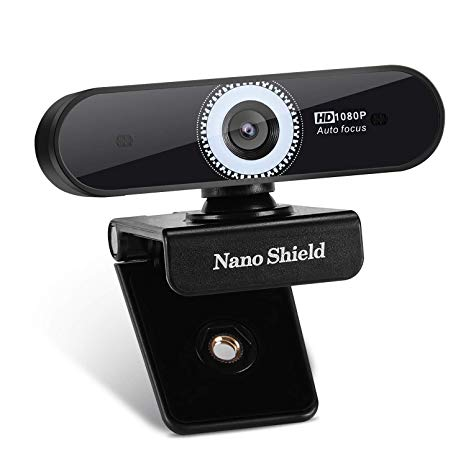
\includegraphics[width=.5\textwidth]
    {images/Alzahraa/webcamera_nano.jpg}%
    \caption[Camera Nano]{1080P Nano Shield N920 Webcamera}\label{fig:nano_webcam}%
  \end{figure}
   \end{enumerate}
   
%%%%%%%%%%%%%%%%%%%%%%%%%%%%%%%%%%%%%%%%%%%%%%%%%%%%%%%%%%%%%%%%%%%%%%%%%%%%
   \section{Software Components}
\subsection{Web Sever}
\hspace{2cm}The aim of this part is to develop website that process requests and delivers data from and to clients over the internet or a local network. A web-based interface is developed for clients to interact with the system. 

\subsection{Robot Software Platform}
\hspace{2cm}We integrate all components of the robot platform using Robot Operating System (ROS). The aim of this part is to provide low-level device control, connect all processes together and provide message-passing between processes with no effort. 